\documentclass[a4paper, 12pt, twoside]{book}

\usepackage[utf8]{inputenc}

\usepackage{verbatim}
\usepackage{color}
\usepackage{graphicx}
\usepackage{array}
\usepackage[top=25mm,bottom=25mm,left=30mm,right=15mm]{geometry}
\linespread{1.1}
% First paragraph indents
% \usepackage{indentfirst}
\setlength{\parindent}{1.5em}
\setlength{\parskip}{1ex plus 0.5ex minus 0.2ex}
\usepackage{listings} % nice source code formatting
\usepackage{color}
\usepackage{amsmath}
\usepackage{url} % make URLs clickable
\usepackage{float}
\usepackage[T1]{fontenc}
\usepackage{todonotes}
\usepackage{setspace}
\usepackage{fancyhdr} % better page headers and footers, http://texblog.org/2007/11/07/headerfooter-in-latex-with-fancyhdr/	
\DeclareUnicodeCharacter{00B0}{\degree}
\usepackage{lipsum}
\usepackage{glossaries}
\makeglossaries
\pagestyle{fancy}
\synctex=1

\fancyhead[ELH]{\slshape \leftmark}
\fancyhead[ORH]{\slshape \rightmark}
\fancyhead[ERH,OLH]{}

\setlength{\headheight}{15pt}


\definecolor{dkgreen}{rgb}{0,0.6,0}
\definecolor{gray}{rgb}{0.5,0.5,0.5}
\definecolor{dkgray}{rgb}{0.3,0.3,0.3}
\definecolor{ltgray}{rgb}{0.8,0.8,0.8}
\definecolor{mauve}{rgb}{0.58,0,0.82}

\lstset{ %
  language=html,                % the language of the code
  basicstyle=\footnotesize,           % the size of the fonts that are used for the code
  numbers=left,                   % where to put the line-numbers
  numberstyle=\small\color{ltgray},  % the style that is used for the line-numbers
  stepnumber=1,                   % the step between two line-numbers. If it's 1, each line 
                                  % will be numbered
  numbersep=10pt,                  % how far the line-numbers are from the code
  backgroundcolor=\color{white},      % choose the background color. You must add \usepackage{color}
  showspaces=false,               % show spaces adding particular underscores
  showstringspaces=false,         % underline spaces within strings
  showtabs=false,                 % show tabs within strings adding particular underscores
  %frame=single,                   % adds a frame around the code
  rulecolor=\color{black},        % if not set, the frame-color may be changed on line-breaks within not-black text (e.g. commens (green here))
  tabsize=2,                      % sets default tabsize to 2 spaces
  captionpos=b,                   % sets the caption-position to bottom
  breaklines=true,                % sets automatic line breaking
  breakatwhitespace=false,        % sets if automatic breaks should only happen at whitespace
  title=\lstname,                   % show the filename of files included with \lstinputlisting;
                                  % also try caption instead of title
  keywordstyle=\color{blue},          % keyword style
  commentstyle=\color{dkgreen},       % comment style
  stringstyle=\color{mauve},         % string literal style
  escapeinside={\%*}{*)},            % if you want to add a comment within your code
  morekeywords={*,...}               % if you want to add more keywords to the set
}

% Tables
\newcolumntype{L}[1]{>{\raggedright\let\newline\\\arraybackslash\hspace{0pt}}m{#1}}
\newcolumntype{C}[1]{>{\centering\let\newline\\\arraybackslash\hspace{0pt}}m{#1}}
\newcolumntype{R}[1]{>{\raggedleft\let\newline\\\arraybackslash\hspace{0pt}}m{#1}}
% Hyphenation
\hyphenpenalty=9000
\righthyphenmin=3
\lefthyphenmin=4

% Hyperlinks
\ifpdf
	\usepackage[pdftex]{hyperref}
\else
	\usepackage{hyperref}
\fi
\hypersetup{
	unicode=true,
	pdftitle={},
	pdfauthor={},
	pdfkeywords={},
	colorlinks,
	citecolor=black,
	filecolor=black,
	linkcolor=black,
	urlcolor=dkgray
}

\bibliographystyle{unsrt}

%### acronyms
\newacronym{GUI}{GUI}{Graphical User Interface}
\newacronym{RPC}{RPC}{Remote Procedure Call}
\newacronym{XMPP}{XMPP}{Extensible Messaging and Presence Protocol}
\newacronym{DOM}{DOM}{Document Object Model}
\newacronym{JSON}{JSON}{JavaScript Object Notation}


\begin{document}
\include{INP-00-glossary}
\pagenumbering{roman}
	%!TEX root = Thesis.tex
\begin{titlepage}

\begin{center}

% Logos
\begin{minipage}{0.30\textwidth}
	\begin{flushleft}
			
\includegraphics[scale=0.45]{images/tud_logo}
	\end{flushleft}
\end{minipage}

\begin{bfseries}
	\large Chair of Computer Networks
		%\textsc{Technische Universität Dresden}\\
		%\textsc{Fakultät Informatik}\\[1em]
\end{bfseries}
    %\Large  \textsc{Chair of Сomputer Тetworks}

%\vspace*{45mm}
\vspace*{75mm}

{\LARGE \bf Master Thesis}\\[1 cm]

\begin{minipage}{0.8\textwidth}
	\begin{center}

		\doublespacing{\Large Generic Frontend for Exploring Sensor and Information Services}\\[3cm]
	\end{center}
\end{minipage}

\vspace{30mm}

% Author and supervisor
\begin{minipage}{0.35\textwidth}
	\begin{flushleft} \large
		\emph{Author:}\\
		M.Sc. Uliana Andriieshyna\\
		Matrikel-Nr: 3828303\\
		~\\ ~\\
	\end{flushleft}
\end{minipage}
\begin{minipage}{0.60\textwidth}
	\begin{flushright} \large
		\emph{Supervisors:} \\
		Dr.-Ing. Josef Spillner\\
		Prof. Dr. rer. nat. habil.\\ Dr. h. c. Alexander Schill\\
		\end{flushright}
\end{minipage}

\vfill

April 10, 2014

\end{center}
\end{titlepage}
% empty page hack
\newpage
\thispagestyle{empty}
\mbox{}

% empty page hack
\newpage
\begin{figure}[h!]
\centering
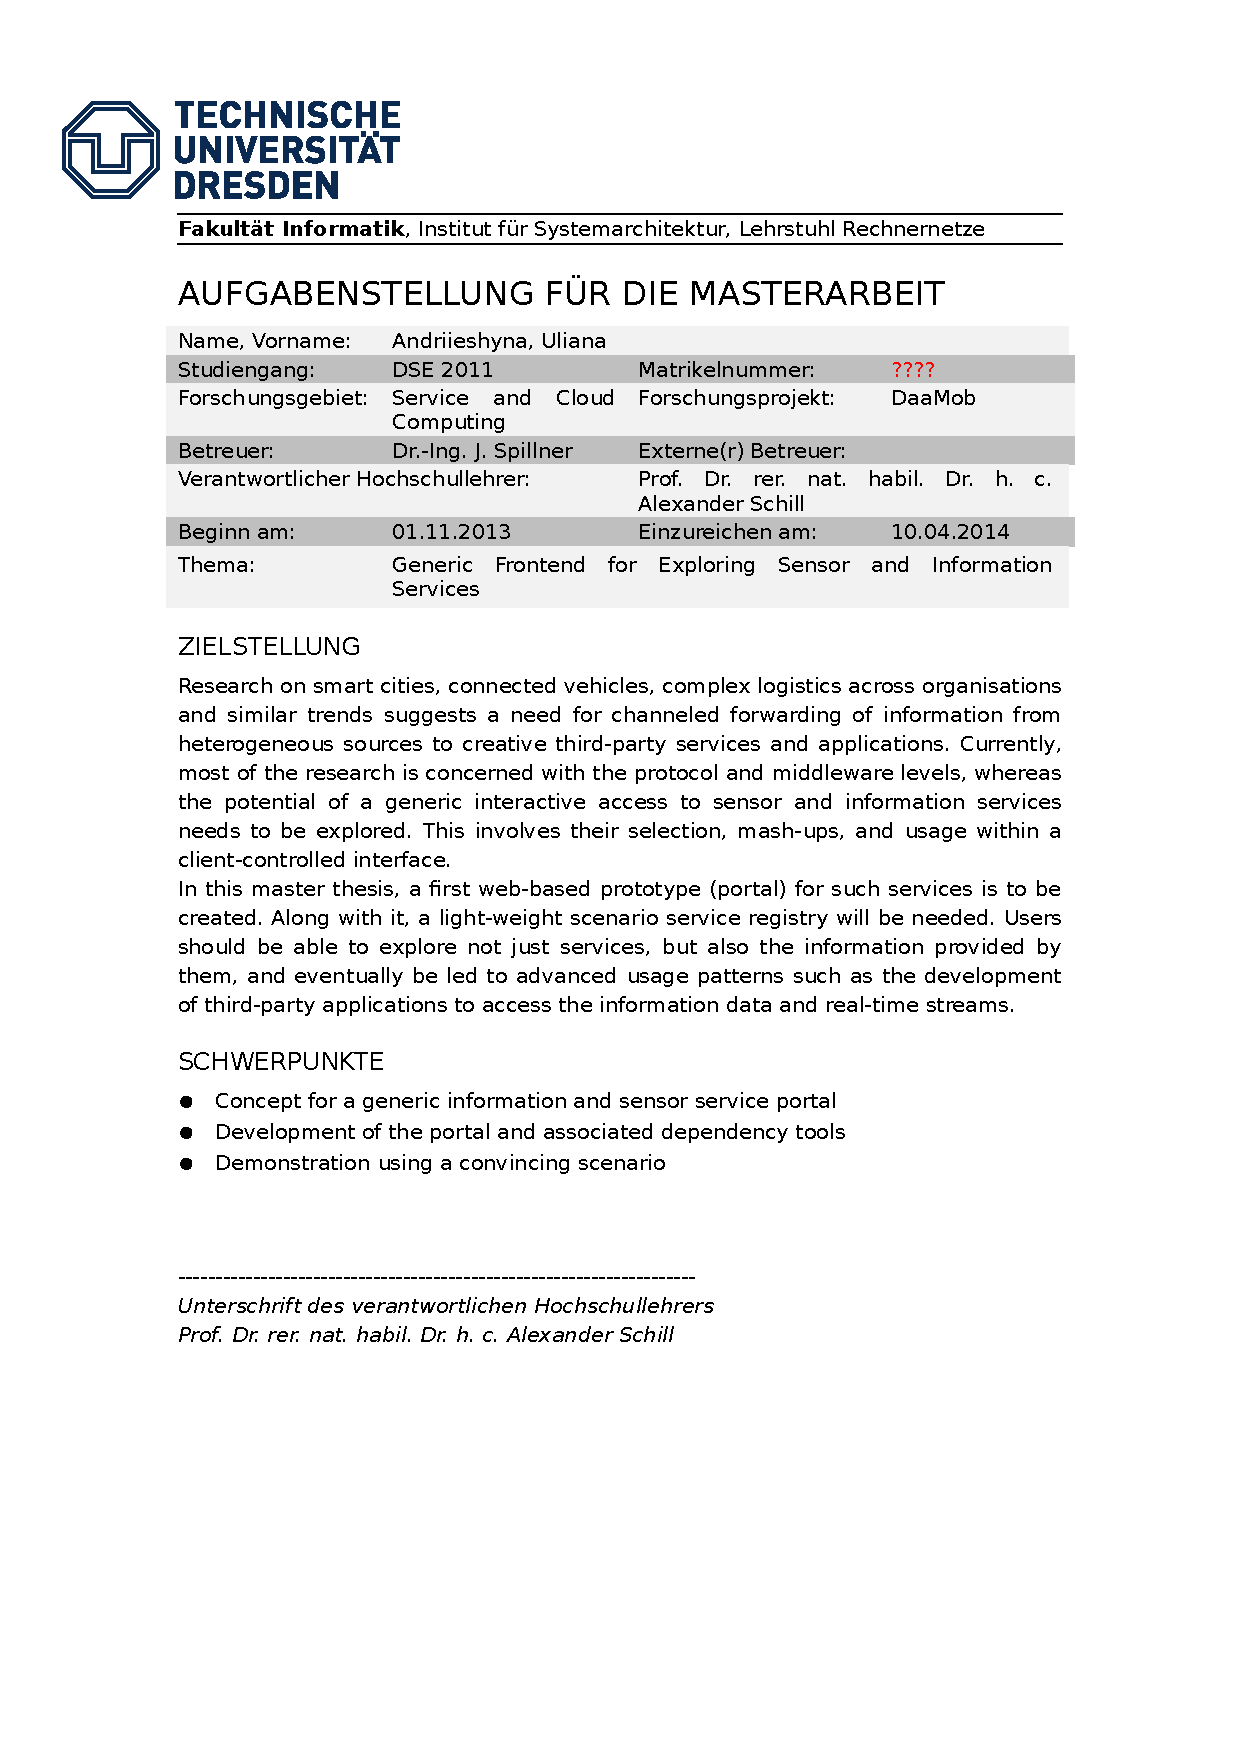
\includegraphics[scale=0.9]{images/AUFGABENSTELLUNG_Uliana.pdf}
\end{figure}
\thispagestyle{empty}
\mbox{}

\newpage
\thispagestyle{empty}
\mbox{}
% Selbständigkeitserklärung
\newpage
\thispagestyle{empty}
\begingroup
  \vspace*{50 mm}
  {\huge \bf Declaration of Authorship}
  \vspace{10 mm}

  I, Uliana Andriiehyna, declare that this thesis, titled "Generic Frontend for Exploring Sensor and Information Services", and the work presented in it have been done on my own without assistance. All information directly or indirectly taken from external sources is acknowledged and referenced in the bibliography.

  \vspace{10 mm}

  Dresden, 10.04.2014 \hspace{6.0 cm} \makebox[1.5in]{\hrulefill}
\endgroup


% empty page hack
\newpage
\thispagestyle{empty}
\mbox{}
\clearpage

\tableofcontents

% empty page hack
\newpage
\thispagestyle{empty}
\mbox{}
\clearpage

\pagenumbering{arabic}
\setcounter{page}{1}
	%!TEX root = Thesis.tex

\chapter{Introduction}

  \begin{singlespace}
     The increasing numbers of sensor devices has increased the number of sensor-specific protocols, platforms and software. The definition "sensor" consists not only a physical device that can be an actuator or measuring device, but also a context-depending information that are available through the Web, e.g. Facebook, Tweets, RSS Feeds, Weather Forecast and etc as a real-time data streaming. As a result various approaches have been proposed to interconnect, maintain and monitor various type of data sources\cite{6588063,bendel2013service,song2010real}.That specifically focused on a platform development, protocol definition and software architecture for the concrete user-oriented requirements and for a narrowly focused areas of usage instead of defining a common system approach. Mainly in proposed approaches was discovered such type of questions as security and privacy between sensor-specific protocol and platform, platform development itself, online aggregation and monitoring of different data sources, social dimensions\cite{eggert2013sensorcloud}, that do not cover criteria of a user-friendly interface, which is for user nowadays an essential part of opportunity to explore a system. Therefore the area of research of this master thesis is dedicated to define common approach of a generic frontend together with a Graphical User Interface(GUI) for exploring data sources, that can be easily and universally interconnected to any platform or a system, which has no GUI. The following sections ground the motivation of the chosen research field, define the central research questions and goals of this master thesis, and describe the overall structure of the work.
  \end{singlespace}

\section{Motivation}
     In the recent years with the technological progress in the information systems, web technologies and in particular sensor data systems, have become an essential part in daily life of the modern society. More and more aspects of human life are shifted to the Web and mobile applications. This allows fast and easy way to get information from any point on earth by using any web, mobile, traditional desktop clients. In the same time have increased a range of sensor specific platform and interfaces. People have started to use them more often not only for manufacture, business, education but also for private reasons. Currently, most of researches is concerned with the protocol and middleware levels, whereas the potential of a generic interactive access to sensor and information services needs to be explored in a best comfortable way for a third-party user, for developer of a such system itself and future application consumer developer. As was already mentioned, most of the works in this area are focused mainly only on a backend side, thus an essential goal fo this thesis is to provide simple and universal for integration web-based generic frontend with a main focus on a dynamic GUI generation. Users and developers should be able to explore not only information provided by Web services, but also from a real sensors around them. The system architecture of such a concept should be distributed in such a way, that already implemented projects could easily interconnect with it.

     Creating composite third-party services and applications from reusable components is an important technique in software engineering and data management. Although a large body of research and development cover integration at the data and platform levels, weak work has been done to facilitate it at generic level. This master thesis discusses the existing web frameworks and component technologies used on presentation level integration, illustrates their strengths and weaknesses, and presents some opportunities for future work. Real-time web applications are connection-oriented applications, with web-based user interfaces, that display information as soon as it was published. Examples include social news aggregators and monitoring tools that continually update themselves with data from an external source.

\section{Application Area}
     In order to define concrete research questions, it is important to determine which kind of concept is going to be proposed and implemented, as well as to clarify the common terms which are used throughout the thesis:
     \begin{itemize}
          \item \textbf{Application.} This thesis is focused on a generic multi-tier web-based frontend that delivers dynamic real-time content to end-users via user-friendly graphical interface. Such type of universal frontend acts as middleware between provider-specific data source and a user. By supporting a concept architecture any backend system can easily send data to the user, without needs to implment a specific frontend.

          \item \textbf{Infrastructure.} Implies a virtualized system architecture of a concept and an application stack required for running an application of the respective prototype, based on 3-tier architecture.

          \item \textbf{Tools and Protocols.} Assumes a set of web-based frameworks and Internet of Things(IoT) protocols for real-time data streaming of a wide range of resources used to explore and maintain services of the aforementioned application.
     \end{itemize}


\section{Research Questions and Goals}
       As mentioned in the previous section, there are already exist a lot of solutions for creating sensor-aware applications. But such type of platforms are focused on a single area of usage and they are not commonly suitable to support the dynamic and adaptable composition of different type of data sources in one dashboard.

       Within this thesis the following research questions should be answered in order to design, implement and evaluate a generic frontend for retrieving data sources: 
       \begin{itemize}
       \item Which architecture should have a concept of a generic frontend?
       \item How should it be designed in order to provide ease of integration with any backend system?
       \item What type of data sources have to be retrieved and what is the most universal interface for collaboration between backend and frontend systems?
       \item How can be a generic GUI designed and implemented by providing dynamic content retrieving?
       \item Which protocol can perform real-time data streaming independently from type of data in it?
       \item Which software components might be applied to the concept in order to be applicable to the most available data sources and platform?
       \end{itemize}

     Therefore, this thesis is aimed at the development of a concept that provides users a possibility to personalize their current environment indepently from any type and kind of surrounding sensors. And provide concept of a generic frontend which can be easily interconnected through the supported interface and extensions points with each other.

\section{Structure}

After the introduction in \emph{Chapter 1} the thesis is structured in the following way:

\emph{Chapter 2} defines the background of the master's thesis, describes the basics of used terminologies and the foundation platforms. Requirements to a concept of a generic frontend that has to be developed are also introduced in this chapter.

\emph{Chapter 3} is devoted to the state of the art analysis. Related research and consumer-based works in the area of sensor-based data retrieving approaches, such as: portal and mashup systems, the browser based and non-browser based systems are investigated and evaluated against the defined requirements.

\emph{Chapter 4} focuses on the concept of the generic frontend for exploring sensor and Information services, considering possible approaches, strategies, web frameworks and necessary criteria, defined in \emph{Chapter 3}.

\emph{Chapter 5} provides the implemented functionality of the concept and evaluated by using convinsing scenario. An example of use case scenario are proposed, described and performed in order to cover the fulfillment of the defined requirements by the developed solution. Important methods and extensions of a an interface are described in details.

\emph{Chapter 6} concludes the master's thesis underlining and evaluating achieved goals and providing prospects for the possible future work.  

	%!TEX root = Thesis.tex
\chapter{Foundations and Requirements Analysis}

\section{Terminology}
The fundamental terms used in this thesis are described below for better under-
standing of the presented research work.
\subsection {Portal}
\subsection {Mashup}

\section{Web-based Frontend Development Framework Analysis}
 \begin{itemize}
\item Bootstrap
\newline
Bootstrap is definitely the most popular and widely used framework, nowadays. It’s a beautiful, intuitive and powerful web design kit for creating cross browser, consistent and good looking interfaces. It offers many of the popular UI components with a plain-yet-elegant style, a grid system and JavaScript plugins for common scenarios.

It is built with LESS and consists of four main parts:

Scaffolding – global styles, responsive 12-column grids and layouts. Bear in mind that Bootstrap doesn’t include responsive features by default. If your design needs to be responsive you have to enable this functionality manually.
Base CSS – this includes fundamental HTML elements like tables, forms, buttons, and images, styled and enhanced with extensible classes.
Components – collection of reusable components like dropdowns, button groups, navigation controls (tabs, pills, lists, breadcrumbs, pagination), thumbnails, progress bars, media objects, and more.
JavaScript – jQuery plugins which bring the above components to life, plus transitions, modals, tool tips, popovers, scrollspy (for automatically updating nav targets based on scroll position), carousel, typeahead (a fast and fully-featured autocomplete library), affix navigation, and more.
\item Foundation
\newline
Foundation is a powerful, feature-rich, responsive front-end framework. With Foundation you can quickly prototype and build websites or apps that work on any kind of device, with tons of included layout constructs, elements and best practices. It’s built with mobile first in mind, utilitizes semantic features, and uses Zepto instead of jQuery in order to brings better user experience and faster performance.

Foundation has a 12-column flexible, nestable grid powerful enough to let you create rapidly multi-device layouts. In terms of features it provides many. There are styles for typography, buttons, forms, and various navigation controls. Many useful CSS components are provided like panels, pricing tables, progress bars, tables, thumbnails, and flex video that can scale properly your video on any device. And, of course, JavaScript plugins including dropdowns, joyride (a simple and easy website tour), magellan ( a sticky navigation that indicates where you are on the page), orbit (a responsive image slider with touch support), reveal (for creating modal dialogs or pop-up windows),  sections (a powerful replacement for traditional accordions and tabs), and tooltips.
\item GroundworkCSS
\newline
GroundworkCSS is a new, fresh addition to the front-end frameworks family. It’s a fully responsive HTML5, CSS and JavaScript toolkit built with the power of Sass and Compass which gives you the ability to rapidly prototype and build websites and apps that work on virtually any device.

It offers an extremely flexible, nestable, fraction-based, fluid grid system that makes creating any layout possible. GroundworkCSS has some really expressive features like tablets and mobile grids which maintain the grid column structure instead of collapsing the grid columns into individual rows when the viewport is below 768 or 480 pixels wide. Another cool feature is a jQuery ResponsiveText plugin which allows you to have dynamically sized text that adapts to the width of the viewport: extremely useful for scalable headlines and building responsive tables.

The framework includes a rich set of UI components like tabs, responsive data tables, buttons, forms, responsive navigation controls, tiles (a beautiful alternative to radio buttons and other boring standard form elements), tooltips, modals, Cycle2 (a powerful, responsive content slider), and many more useful elements and helpers. It also offers a nice set of vector social icons and a full suite of pictographic icons included in FontAwesome.

To see the framework in action you can use the resizer at the top center of the browser window. This way you can test the responsiveness of the components against different sizes and viewports while exploring the framework’s features.

GroundworkCSS is very well documented with many examples, and to get you started quickly the framework also provides you with several responsive templates. The only thing I consider as a weakness is the missing of a way to customize your download.

http://usablica.github.io/front-end-frameworks/compare.html

\item Gumby
\newline
Gumby is simple, flexible, and robust front-end framework built with Sass and Compass.

Its fluid-fixed layout self-optimizes the content for desktop and mobile resolutions. It support multiple types of grids, including nested ones, with different column variations . Gumby has two PSD templates that get you started designing on 12 and 16 column grid systems.

The framework offers feature-rich UI Kit which includes buttons, forms, mobile navigation, tabs, skip links, toggles and switches, drawers, responsive images, retina images, and more. Following the latest design trends the UI elements have Metro style flat design but you can use Pretty style with gradient design too, or to mix up both styles as you wish. An awesome set of responsive, resolution independent Entypo icons, for you to use in your web projects, is completely integrated into the Gumby Framework.

Gumby has also a very good customizer with color pickers which helps you to build your custom download with ease.
\item Kube
\newline
Lastly, if you need a solid, yet simple base without needless complexity and extras, for your new project, Kube can be the right choice. Kube is a minimal, responsive and adaptive framework with no imposed styling which gives you the freedom to create. It offers basic styles for grids, forms, typography, tables, buttons, navigation, and other stuff like links or images.

The framework contains one compact CSS file for building responsive layouts with ease and two JS files for implementing tabs and buttons in your designs. If you are looking for maximum flexibility and customization, you can download developer version which includes LESS files, with variables, mixins and modules.
\end{itemize}

\begin{figure}[!ht]
\centering

\includegraphics[scale=0.7]{images/Bootstrap&Foundation.png}
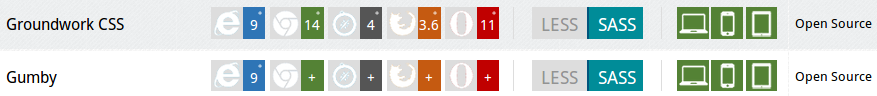
\includegraphics[scale=0.7]{images/Groundwork&Gumby.png} 

\includegraphics[scale=0.7]{images/Kube.png}  
\caption[Framework Comparison]{Framework Comparison}
\label{img:Bootstrap&Foundation.png}
\label{img:Groundwork&Gumby.png}   
\label{img:Kube.png}                          
\end{figure}
\footnotetext{Image taken from \url{http://usablica.github.io/front-end-frameworks/compare.html}}

\section{Summary}
In this master thesis, a first web-based prototype (portal) for such services is to be
created. Along with it, a light-weight scenario service registry will be needed. Users
should be able to explore not just services, but also the information provided by
them, and eventually be led to advanced usage patterns such as the development
of third-party applications to access the information data and real-time streams.
\section{Basic Functionalities}


	%!TEX root = Thesis.tex
\chapter{State of the Art}
The following chapter covers an overview and analysis of the existent solutions in
the related research areas of web-based third-party applications, which were designed specially for retrieving differet type of sensed data to the user. At the beginning the prominent examples of dashboards platforms are studied and evaluated against the requirements described in the previous chapter with a purpose to clarify their individual capabilities.

\section{?Web of Sensors?}
 Since the thesis is targeted at the creation of a generic user-friendly data stream interaction system and currently every project focused on a specific area of realization and concrete sensor types, such as urban environment\cite{song2010real}. The real-time environmental monitoring portal or geospatial infrastructure for effectively or  efficiently collecting and serving vast field data over the web. Internet based urban environment observation system that can real-time monitor environmental changes of temperature, humidity, illumination or air components in urban area. It provides web-based platform, where end-user can simply monitor urban area in his/her city. In environmental monitoring, the field server for constructing outdoor sensor network is a Web-based field observation device, which detects field environmental parameters and publishes them on Internet in real-time.
\newline
	\emph{Smart city}\cite{6588063}tool using information technology and communication (ICT) to help local government to monitoring what currently happened in the city. pplication for monitoring city in single dashboard to help summarize the current condition of city. The architecture system use network sensor consisting of sensor nodes that has function to capture city condition like temperature, air pollution, water pollution, traffic situation. Also we can add another information socio-economic situation like public health service, economic indicator, energy supplies, etc. We have successfully developed the prototype of the smart city dashboard the give more accurate information of Bandung City, one of big cities in Indonesia. This study has implemented prototype system of smart city dashboard at Bandung. It consists of network sensor, server, application and also communication protocol which is used for city monitoring. The summary information of city can be displayed in single view to help people watching, analyzing and action to what being happen at the real-time in the city.
\newline
	\emph{Microsoft SensorMap\cite{nath2007sensormap}}has proposed a system to monitor and present physical sensors in the real world. SensorMap allows owners of sensor networks to register their physical sensors and publish their data on SensorMap. They use GeoDB to store the sensor network information, DataHub to retrieve the new sensor data to enable real time services, and the aggregator to summarize sensor data in a specific area to clients.
\newline
	 \emph{LiveWeb Portal}\cite{yang2011liveweb} presents the architecture, design, and application of a sensorweb service portal, where sensorweb is a global observation system for varied sensory phenomena from the physical world and the cyber world. This system has been used to represent and monitor real-time physical sensor data and cyber activities from ubiquitous sources. LiveWeb meets its goal of providing an efficient and robust sensor information oriented web service, enabled with real-time data representation, monitoringand notification.LiveWeb has the following properties: the system enables sensorweb service accessible from anywhere, makes sensor network data readable by anyone, sensor network sharing, the system make sensor data format transparent to data users, real-time data display suits sensor data properties, an offline alert system strengthens real-time features.
\newline
	\emph{Internet of Things}\cite{bendel2013service} where presented a service platform based on the Extensible Messaging and Presence Protocol (XMPP) for the development and provision of services for Internet of Things(IoT) mainly focusing on the integration of things based on service technologies, scenarios in domains like smart cities, automotive or crisis management require service
	platforms involving real world objects, backend-systems and mobile devices. And argued necessary usage of
    XMPP client as protocol for unified, real-time communication and introduce the major concepts of our platform. Based on two case studies we demonstrate real-time capabilities of XMPP for remote robot control and service development in the e-mobility domain.
 \newline
	 \emph{Dynvoker Portal}\cite{spillner2008ad} a generic human-driven ad-hoc usage approach, by including rapid service testing and dynamic inclusion of services as plugins into applications. Dynvoker consists of a relatively small application core which can be run as a servlet, a web service or a command-line application. explore method-centric and resource-centric services alike, output forms in various formats or integrate GUI services to provide a richer user experience. The generic design of many parts of Dynvoker has yielded a lightweight architecture which is freely available to any interested person as an open source project.
\newline
	\emph{Sensor Web Enablement} project\cite{ogc} is focused on developing standards to enable the discovery of sensors and corresponding observations, exchange, and processing of sensor observations, as well as the tasking of sensors and sensor systems.
	 Open Geospatial Consortium, Inc. members specifies interoperability interfaces and metadata encodings that enable real time integration of heterogeneous sensor webs into the information infrastructure. Developers will use these specifications in creating applications, platforms, and products involving Web-connected devices such as flood gauges, air pollution monitors, stress gauges on bridges, mobile heart monitors, Webcams, and robots as well as space and airborne earth imaging devices. In this publication by OGC was defined such an important XML-based standatrds as: Sensor Model Language (SensorML), Sensor Observation Service (SOS), Web Notification Service (WNS) etc. As subproject calls SANY(Sensors Anywhere) focuses on interoperability of in-situ sensors and sensor networks. The goal for the SANY architecture is to provide a quick and cost-efficient way to reuse data and services from currently incompatible sensors and data sources in future environmental risk management applications. By developing a standard open architecture and a set of basic services for all kinds of sensors, sensor networks, and other sensor-like services, the SANY IP supports and enhances both GMES (Global Monitoring for Environment and Security, a major European space initiative) and GEOSS (Global Earth Observation System of Systems) in the area of in-situ sensor integration. Though the SANY work enhances interoperability for monitoring sensor networks in general, the application focus is on air quality, bathing water quality, and urban tunnel excavation monitoring.
\newline 
    \emph{VICCI Project}(Visual and Interactive Cyber-physical Systems Control and Integration)\cite{vicci}. The scope includes smart home environments and supporting people in the ambient assisted living, considers the software-technical side of so-called “Cyber-physical systems” (CPS). This term includes complex, embedded systems, which connect the virtual and the physical world with each other (IoT)in different application scenarios. The main uses of CPS are in logistics, traffic optimization, in the use of robots in the industrial and domestic sectors, in modern energy networks (Smart grid), in the building and factory automation (Smart factory), as well as in the field of intelligent office installations (Smart Office). The aim of project VICCI is the creation of software engineering principles that are necessary for the development of complex cyber-physical systems. Firstly, CPS should be made understandable and accessible by means of a comprehensive control centre. Secondly, platforms that enable the development and marketing of software for complex CPS through a pure control panel are to be developed. A domestic environment is considered a sample scenario in which a person with reduced mobility is supported by sensors, actuators and a service robot, which is currently seen as a complex cyber-physical system. No concreate frontend or any kind of user-friendly have been not yet developed. 
\newline
	A series of articles devoted to integrate sensed data into a Cloud. Special attention is given to privacy-relevant or otherwise sensitive information that stores in Cloud. SensorCloud\cite{hummen2012cloud}, a cloud design for user-controlled storage and processing of sensor data proposed security architecture enforces end-to-end data access control by the data owner reaching from the sensor network to the Cloud storage and processing subsystems as well as strict isolation up to the service-level. In this paper authors implement transport security mechanisms for communication with the Cloud, applies object security mechanisms to outbound data items, and performs key management for authorized services. \emph{CloudRemix\cite{spillner2013personal}} a Personal and Federated Cloud Management Cockpit, an interactive cockpit to manage personal clouds and their federations. Is a new techniques for users to perform asset discovery, exchange and management in Cloud area. The CloudRemix prototype demonstrates its utility to manage personal clouds in both social and market-driven environments. The goal of CloudRemix is to be open, user-centric regarding the manageable assets, and flexible regarding their free or commercial exchange, with or without explicit contract negotiation. CloudRemix is an open-source web-based cockpit application with support for multiple users. Each user gets to see an aggregated list of both local and remote services of each of the asset types.


\section{Frontend Development Approaches}
In computer science, the frontend is responsible for collecting input from user and processing it to a backend system and another direction - collecting data from backend, namely sensor data steam, and processing it to the user-friendly interface. Therefore, on the one side, generic frontend has to satisfy architecture requirements from backend, such as: fine-grained distributred structure, cross-platforming, multy-user capabilities; and on the other side, define a dynamic user-friendly interface to a end-user. And to satisfy aforementioned requirements from backend server it is necessary to compare all available web-based applications.
\newline
To retrieve sensor data from different resources in one web-based interface existent next approaches :
\begin{itemize}
 \item portal with portlets,
 \item mashup\footnote{\url{http://www.programmableweb.com/applications}},
 \item HTML5 technology
\end{itemize}
%Portal
Portal technology brings information together from diverse sources in a uniform way. Usually, each information source gets its dedicated area on the page for displaying information (a portlet); often, the user can configure which ones to display. The extent to which content is displayed in a 'uniform way' may depend on the intended user and the intended purpose, as well as the diversity of the content. Very often design emphasis is on a certain 'metaphor' for configuring and customizing the presentation of the content and the chosen implementation framework and/or code libraries\cite{pautasso2008restful,seong2006usability}. In portal technologies end-user can customize number of retrieved data sources, but for that he has to be aware what is it and how to integrate it in portal. User interface in portals have fixed layout, style and location on the web page. To make changes in it, end-user needs to have a deep knowlendge of the system architeture and of whole portal entirely.
 \newline
%Mashup
Mashup is a web page, or web application, that uses content from more than one source to create a single new service displayed in a single graphical interface. The term implies easy, fast integration, frequently using open application programming interfaces (API) and data sources to produce enriched results that were not necessarily the original reason for producing the raw source data. The term mashup originally comes from pop music, where people seamlessly combine music from one song with the vocal track from another-thereby mashing them together to create something new. The main characteristics of a mashup are combination, visualization, and aggregation. It is important to make existing data more useful, for personal and professional use. To be able to permanently access the data of other services, mashups are generally client applications or hosted online.
Both commercial products and research prototypes have a broad range of features that simplify a mashups design process, and provide mashups storage and publication. But to customize retrived resources end-user have no option, as use only predefined type and numbers of applications, that was created by application or platform developer. Also Mashup approach is strictly platform- and customer-oriented. It is simply provides stack of tools, by using which user through an user-friendly interface 
The architecture of a mashup is divided into three layers:
 \newline
 \begin{itemize}
\item \emph {Presentation / user interaction:} this is the user interface of mashups. The technologies used are HTML/XHTML, CSS, Javascript, Asynchronous Javascript and XML (Ajax).
 \newline
\item \emph {Web Services:} the product's functionality can be accessed using API services. The technologies used are XMLHTTPRequest, XML-RPC, JSON-RPC, SOAP, REST.
 \newline
\item \emph {Data:} handling the data like sending, storing and receiving. The technologies used are XML, JSON, KML.
 \newline
 \end{itemize}
Architecturally, there are two styles of mashups: Web-based and server-based. Whereas Web-based mashups typically use the user's Web browser to combine and reformat the data, server-based mashups analyze and reformat the data on a remote server and transmit the data to the user's browser in its final form\cite{bolin2005end}.
 \newline
Mashups and portals are both content aggregation technologies. Portals are an older technology designed as an extension to traditional dynamic Web applications, in which the process of converting data content into marked-up Web pages is split into two phases: generation of markup "fragments" and aggregation of the fragments into pages. Each markup fragment is generated by a "portlet", and the portal combines them into a single Web page. Portlets may be hosted locally on the portal server or remotely on a separate server.
\newline
%HTML5
\section{HTML5 Technology}
To satisfy one of the main requirement about dynamic user-friendly interface, adaptable to any kind of device, mashup architecture should be enhanced with a HTML5 Technology. Based on various design principles, that truly embody a new vision of possibility and practicality\cite{hickson2011html5}.
\begin{itemize}
\item Compatibility(inharit all previous techniques and standards)
\item Utility
\item Secure by Design(origin-based security model that is not only easy to use but is also used consistently by different APIs.)
\item Separation of Presentation and Content(CSS3)
\item Interoperability(Native browser ability instead of complex JavaScript code; a new, simplified DOCTYPE;simplified character set declaration; powerful yet simple HTML5 APIs)
\item Universal Access(suport users with disabilities by using screen readers; media independence-HTML5 functionallity should work across all different devices and platforms; support for all world languages)
\end{itemize}

\section {UI Usability}
ISO defines usability as "The extent to which a product can be used by specified users to achieve specified goals with effectiveness, efficiency, and satisfaction in a specified context of use."
Main goals which user-friendly interface have to satisfy from a user point of view are\cite{baxter2012human,jakob,visdesign}:
\begin{itemize}
\item Clarity: a user have to easy understand what is the content, how to explore content that provided by application and which rights have a user
\item Evidence: accordance of standardized icons, titles, layout (intuitive design)
\item Satisfaction: How pleasant is it to use the design?
\item Adaptivity: nicely feet to a different types of devices
\end{itemize}

\section{Summary}
This chapter briefly introduced main approaches for building web-based dashboards by retriving sensed data. Main focus was given to its multy-user usability, adaptive UI design, dynamic content composition. Where portal and mashup technology come into a picture. 
\begin{figure}[!ht]
\centering
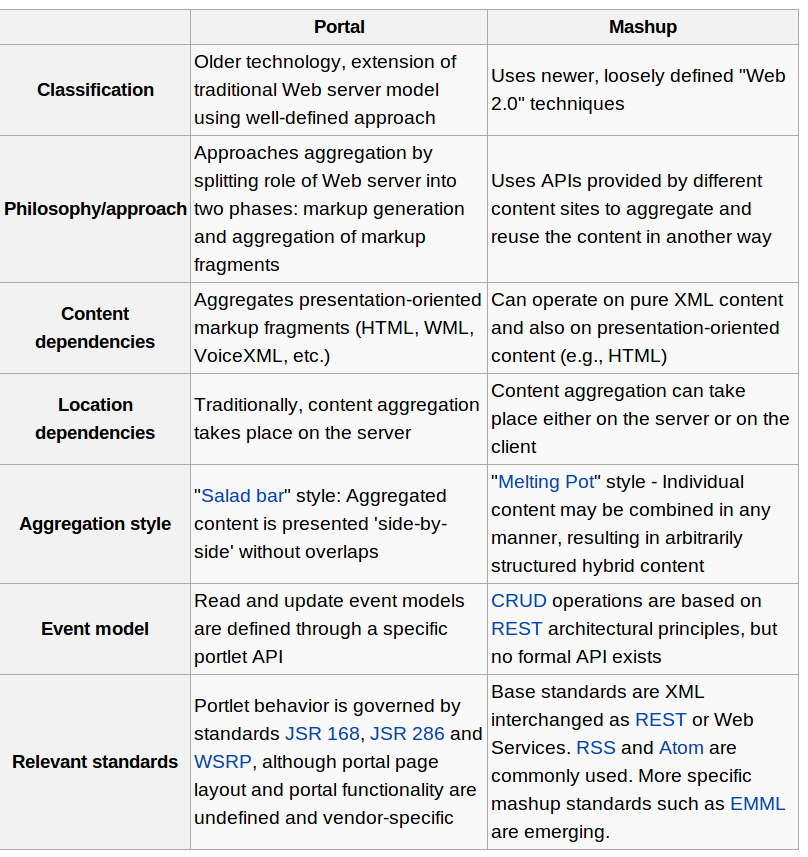
\includegraphics[scale=0.8]{images/MashupVsPortal.png}   
\caption[Comparative Characteristic of Approaches]{Comparative Characteristic}
\label{img:comparative characteristic}                           
\end{figure}

	%!TEX root = Thesis.tex
\chapter{Concept}
     The chapter describes a concept of a user-friendly generic frontend for exploring sensor data, going through a software architecture design and a content aggregation of a web-based user interface controlled and provisioned by end-user requests. The concept is developed based on the analysis of the current state-of-the-art, modern technologies and requirements formulated in the Chapter 2. 

     The Section 4.1 begins this chapter with a software design according to 3-tier architecture, which contains client, application and data tiers. Next sections presents detailed description of an every tier, with corresponding functional modules based on a fine-grained structure. Every part of a system is responsible for providing application functionality of a corresponding tier. Summary of this chapter underlines main responsibility and requirements for every part of the system infrastructure. It clarifies requirements to a prototype implemented in the Chapter 5.


\section{Concept in 3-tier Architecture Projection}

  Building a system architecture based on a fine-grained structure satisfies one of the important requirement defined in the Section 2.1. Such a structure of a generic frontend should be scalable and easily integrated with any kind of a backend, where every module is responsible for its personal independent task. Thus, deployment of new changes to any module have no influnce on another parts of an architecture. System becomes consistent and reliable. An important task is to determine the software design according to 3-tier architecture, where presentation, application processing, and data management functions are logically separated. The multi-tier architecture provides abstract structure of modules and gives a possibility to define in which concrete module of a system developer is interested in. Also it describes how different parts of frontend are connected with each other and which extensions and integration points for backend are available.
  \newline
  The Figure \ref{img:3-tier Architecture} shows the concept infrastructure:

  \begin{itemize}
  \item \textbf{Client Tier:} web-based GUI and client framework;
  \item \textbf{Application Tier:} application logic, interface of communication between tiers, backend integration points;
  \item \textbf{Data Tier:} provides description of data sources based on defined data standard and real-time data streaming of all sensors registered in the system.
  \end{itemize} 

  \begin{figure}[!ht]
  \centering
  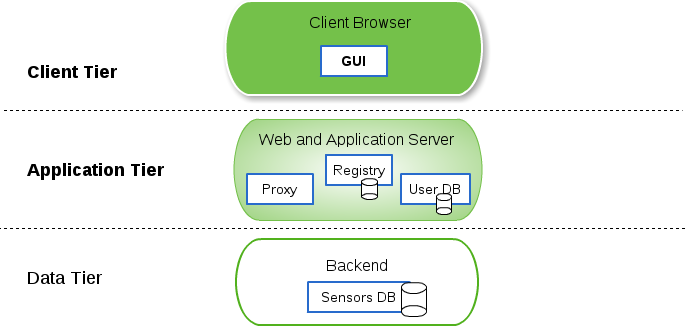
\includegraphics[scale=0.7]{images/3tier.png}   
  \caption[3-tier Architecture]{3-tier Architecture}
  \label{img:3-tier Architecture}                           
  \end{figure}

  \emph{Client Tier} hosts the presentation layer components. The main function of the interface is to translate tasks and results from application tier into a user-friendly GUI via a client framework. This tier was defined in order to satisfy next requirements to the concept: cross-platform application, usability properties and responsiveness of a concept, which is formulated in the Section 2.1.

  \emph{Application Tier} includes business logic and data access tiers. It controls an application's functionality by performing detailed processing, transformation of a one type data to another, defines an interface between the client tier and the data tier. Besides possessing application logic between two another tiers of infrastructure, this tier also contains integration point with a backend system. Loose coupling and multi-user binding is discovered and implemented in this tier.

  \emph{Data Tier} contains source of data that has to be retrieved by the application tier to a client tier, by request from a user. This tier keeps data neutral and independent from application server or business logic. Backend generates a description of a data source in a system-defined way and provides an access to the description and data itself through the standard intreface.

  From a historical perspective the three-tier architecture concept emerged in the 1990s from observations of distributed systems\cite{wiki:3tier} (e.g., web applications) where the client, application and data tiers ran on physically separate platforms. Nowadays, MVC and similar model-view-presenter (MVP) patterns are used for a separation of concerns. It discovers design patterns that apply exclusively to the presentation layer of a large system. In simple scenarios MVC may represent the primary design of a system, reaching directly into the database. This way, to ensure highly adaptive GUI independently from a data and application tiers, MVC pattern comes into a picture. As a part of frontend logic it will be described in the next subsection.
  
  The multi-tier architecture model may seem similar to the model-view-controller (MVC) concept. However, topologically they are different. A fundamental rule in a three tier architecture is the client tier never communicates directly with the data tier; in a three-tier model all communication must pass through the middle tier. Conceptually the three-tier architecture is linear. However, the MVC architecture is triangular: the view sends updates to the controller, the controller updates the model, and the view gets updated directly from the model.

  The next section describes every functional module of a respective tier according to 3-tier architecture.

\section{Client Tier}
  The client or presentation tier a layer which user can directly access from any type of portable device. In the Section 3.2 the necessity to implement web based portable application was proved, so that a user can access it by using browser. This tier consists user-friendly GUI which includes widgets structured according to the responsive layout and client framework. First of all, client tier gives an overview of a design layout (Fig.\ref{img:GUI Mockup}), content provided by data source and managment panel (e.g. technical details of a system architecture such as: end-points configuration, API documentation or SDK downloads). Secondary, it contains a client-based library to bind client and application tier. This tier also responsible for adaptation of a GUI to any kind of mobile or desktop devices. 
  \subsection{Web-based GUI Composition}

  The Figure \ref{img:GUI Mockup} presents a simple content layout that has to be presented on a web-page in order to satisfy all possible user requirements. It contains:

    \begin{figure}[!ht]
    \centering
    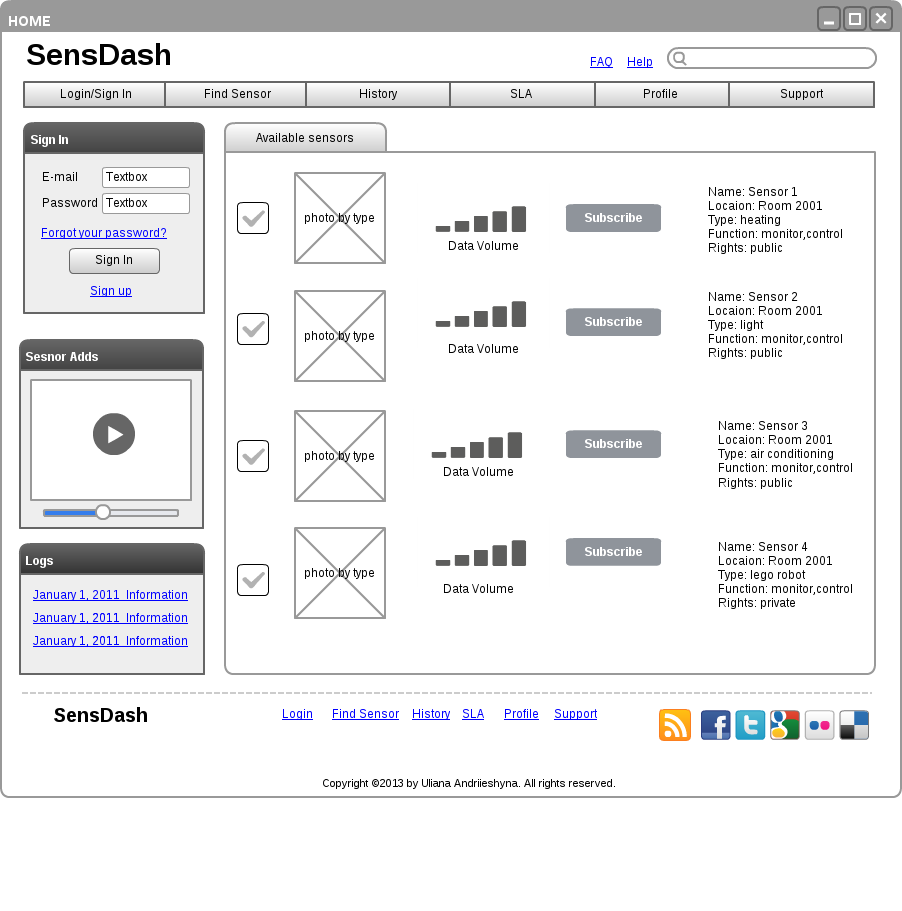
\includegraphics[scale=0.5]{images/Mockup.png}   
    \caption[GUI Mockup]{GUI Mockup}
    \label{img:GUI Mockup}                           
    \end{figure}

      \begin{itemize}
      \item \emph{Main navigation tabs}: a sensors list contains a list of all available sensors; subscriptions - show all data sources to which subscribed by a user; favorites tab saves favorite data sources among already subscribed; in the settings tab a user can manage own profile and also add new sensors by using corresponding form; and the admin references tab clarify steps needed to be established in order to develope own application.
      \item \emph{Log in form} with user name and password. After user logged in, the system defines his/her rights and applies visibility rules according to assigned role. All users can explore description of every data retrieved by system, but only after subscription to a sensor it becomes possible to get real-time streaming data. Users that have admin rights get an interface to manage sensors. Simple user without privileges gets an interface to receive statistic and information from sensors and to maintain his/her own account data.
      \item \emph{Sensor icon} defines what the current type of sensor is, e.g. light, temperature, heating, robot lego battery status etc. It helps easily and quickly understand what is the main function of a sensor in the list.
      \item \emph{Availability or unavailability} of a data source. User can subscribe only to services which are online. If some services become offline it will be automatically marked as inactive and after page reload will be deleted from the list of available sensors. As soon as new data will be sent, a user will immendiatyely see it on the subscriptions tab. If user has already subscribed to any sensor, this sensor automatically added to a list/tab of subscriptions made by user. Also a user can define hierarchy in which sensor information has to be displayed. It is done by using ``favorite'' label/tab. It helps user to receive information from a sensor in a fast way.
      \item \emph{Data Volume icon} shows the average data stream volume needed to retrieve sensor data (Kb/s). User can define his possibilities of getting such type of streaming data according to his Internet connection. Ideally, the dashboard should automatically adapt quality of streaming data based on connection throughput. Not only data volume depends on quality of a service itself, but also security level, reliability and performance. Such type of data description can be substituted by most relative icons such as: ``lock'' icon to define security level or appearance of a reliability label.
      \item \emph{Description and preview}. The best way to give a user full information about data source is to provide a preview or examples of source data. It is not only description but also real-time drawing graphics, real example of video or audio, images etc.
      \item \emph{Access and providers}. Based on provider of a data source, data can be private or public. For public type of data a user do not have to accept any SLA to subscribe to sensor. But for private data it is important to accept SLA between subscriber and provider before user will get any real data.
      \item \emph{Search panel}. Need to filter and search between available sensors, which only based on information available for client tier. Without any queries to application or data tier.
      \end{itemize}

    The general use case is shown on the Figure \ref{img:use_case_basic}. User can use any type of mobile device and his favorite browser to receive information from data sources (sensors) by using web-page as a dashboard. Once a user logs in to the dashboard, he/she can explore all available sensors. If he/she is already a user of the dashboard all his/her preferences will be loaded from a server automatically and appear in respective tabs.

        \begin{figure}[!ht]
        \centering
        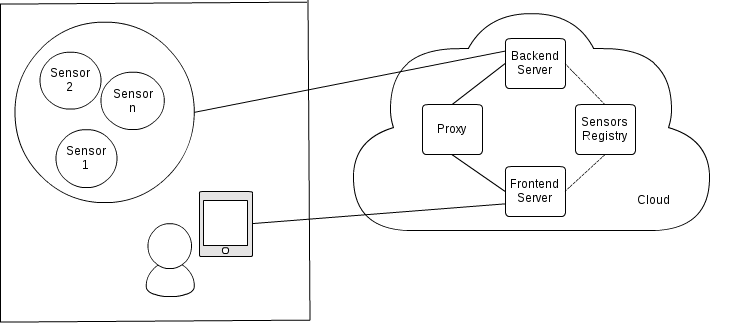
\includegraphics[scale=0.6]{images/User_Case.png}   
        \caption[Use Case]{Use Case}
        \label{img:use_case_basic}                        
        \end{figure}

    \subsection{JavaScript MVC}
    As it was mentioned on the begining of the section, the second responsibility of a client tier is to bind application and client tiers. It can be done by using a client-based framework which is based on the MVC pattern.

    In the design shown on the Figure \ref{img:MVCPattern}, a common Model-View-Controller pattern takes place. Model represents the application object that implements the application data and business logic. The View is responsible for formatting the application results and dynamic page construction. The Controller is responsible for receiving the client request, invoking the appropriate business logic, and based on the results, selecting the appropriate view to be presented to the user. The Model represents data and the business rules that govern access to and updates to this data. A View renders the contents of a Model. It accesses data through the Model and specifies how that data should be presented. It is the View's responsibility to maintain consistency in its presentation when the Model changes. This can be achieved by using a push Model, where the View registers itself with the Model for change notifications, or a pull Model, where the View is responsible for calling the Model when it needs to retrieve the most current data. A Controller translates interactions with the View into actions to be performed by the Model. In a stand-alone GUI client, user interactions could be button clicks or menu selections, whereas in a Web application, they appear as GET request. The actions performed by the Model include activating business processes or changing the state of the Model. Based on the user interactions and the outcome of the Model actions, the Controller responds by selecting an appropriate View.

     \begin{figure}[!ht]
     \centering
     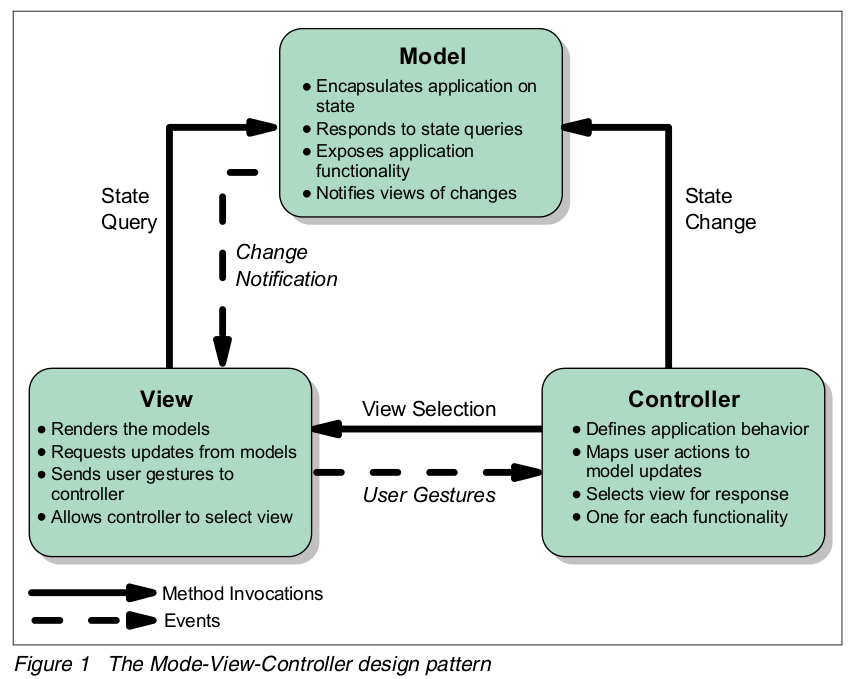
\includegraphics[scale=0.5]{images/MVCPattern.png}   
     \caption[MVC Pattern]{MVC Pattern\footnotetext{Image taken from, \url{blog.csdn.net/cain/article/details/6617173}}}
     \label{img:MVCPattern}                           
     \end{figure}
  
  Not necessary to follow the MVC pattern strictly. The idea is to separate Model, View and application logic for the best separate of concerns.

\section{Application Tier}
  This layer coordinates commands of processes, makes logical decisions and performs calculations. It also moves and processes data between the two surrounding layers.

  Application tier contains all logical modules: Web server, Registry, Data Hub and Web-based Frontend. All these modules connect to each other as shown on the Figure \ref{img:structure}. 
    \begin{figure}[!ht]
    \centering
    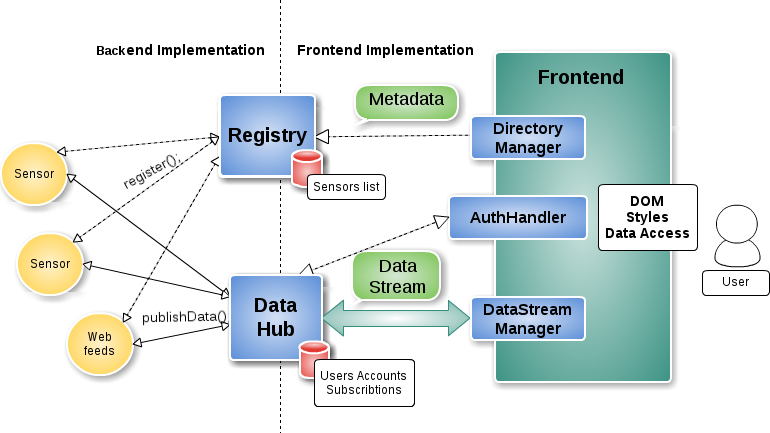
\includegraphics[scale=0.6]{images/Structure.png}   
    \caption[System Architecture]{System Architecture} 
    \label{img:structure}                        
    \end{figure}

    The System Architecture is splitted to a backend and frontend, that gives an overview of how these two parts are connected. Respectively ``backend/frontend implementation'' means that all modules of each side have to be implemented separately. Such module as Registry and Data Hub defined and standardized by frontend, in order to clarify interface of collaboration with backend. Implementation of Registry and Data Hub modules relate to the backend responsibility.

  \subsection{Registry}
    The Registry is a module responsible for storing an info about all registered sensors in order to provide descriptional overview to a user. The Frontend's GUI requests and aggregates information from the Registry about data sources registered in it and dynamically presents it to the user. The Registry contains next necessary attributes: unique id of a sensor, title, description, availability, private or public access description, data provider, service-level agreement (SLA) and its last update time, number of end-points available for one sensor and data format. JSON format fully satisfies described metadata format. The type of connection interface between the Registry and the frontend will be defined in the Section 4.3.3. Structured sensors' attributes within JSON format describes sensors metadata and gives an opportunity to transform it automatically to the graphical container of as a part of the GUI. Registries which provides defined standard can be easily added to the frontend in a runtime. The Registry specifies simple interface schema in JSON format to specify all available attributes and properties. It is a lightweight format, native to browser and much simpler to parse than XML. It separates metadata of a sensor from a real-time data stream. 

    Before publishing data to the Registry, a data publisher, which is a part of a backend, should specify all required fields based on a description of a sensor. An important attribute of a sensor is its ``id'', which in order to avoid inconsistency between different Registries must be unique for every data source. Id can be an alphanumeric scring of arbitary length.

    To get an access to a real-time data streams a user have to be subscribed to it. The process of subscription to a public and private data sources differ. Sensors with a public access do not require explicit SLA accepting, while private data sources obligate a user to accept provider SLA before getting any real-time data. Once a user accepts the corresponding SLA real-time data becomes available as long as the SLA is up-to-date. When the provider of a data source makes changes in the SLA, a user has to be immediately notified and to avoid SLA disagreements automatically unsubscribed from a sensor. The implementation details are described in the Section 5.3.2.

    End-points for a sensor handle real-time data streaming and have to be sctuctured in a heuristic order, in order to switch end-points when another one fails. The number of sensor end-points for data streaming is not limited.

  \subsection{Data Hub}
    Since the the Registry responsible for collecting metadata of sensors, the Data Hub is responsible for mapping interface of particular sensor data stream format into a format supported by the frontend and delivered through the common universal protocol. It means that the Data Hub has to satisfy next requirements:

    \begin{itemize}
    \item be aware of a metadata provided by the Registry to the frontend;
    \item bind metadata from the Registry with real-time data streaming from a sensor;
    \item get and parse sensor streaming data and reconvert it to the type supported by universal protocol;
    \item implement universal protocol to provide exchange message with a server in order to retrieve streaming data from a sensor;
    \item store history from sensors and user personal preferences.
    \end{itemize}
    
    A GUI depends a lot on user personal preferences. It may contain sensor subscriptions list, favorite data sources, user profile and list of available sensors. All these data has to be stored in the Data Hub and loaded after authentication process was sucessfully passed.

  \subsection{Web-based Frontend}
  \label{section:web-frontend}
    \subsubsection{Web server}
    The primary function of a web server is to deliver web content to clients. The communication between client and server takes place using the Hypertext Transfer Protocol (HTTP).

    In proposed concept Web server is responsible for robust and efficient serving of static files (*.html, *.css, *.js etc.). The goal is to exclude dependencies on concrete backend platforms or frameworks and to provide generic frontend as an easily plugable component. Such a common and simplified design makes it possible to extend and scale every part of a distributed system independently. Specific operation logic like authentication of user, registration of sensors and users are delegated to external components such as Registry, Data Hub and Authentication Hadler (AuthHandler), these external components can be interchanged without dependency to the system itself.

    \subsubsection{AuthHandler}
    Authentication Handler (AuthHandler) is responsible for logging in and optionally registering a user in the the system. After a user gets necessary ID and confirms his/her personality using password and name, system automatically applies visibility rules. After verification and confirmation of credentials, stored on Data Hub, it becomes possible to bind user ID with personal preferences. These preferences include: user subscriptions, favorites, social sharing information and session data.

    \subsubsection{Interfaces}
      On the Figure \ref{img:structure} exist 3 communication channels: 
      \begin{itemize}
      \item Registry to Directory Manager (one-way connection);
      \item Data Hub to/from DataStream Handler (asynchronous duplex connection);
      \item Data Hub to/from AuthHandler (synchronous duplex connection). 
      \end{itemize}

      \textbf{Registry to Directory Manager Interface}
      \newline
      The Registry contains pairs of attributes -- values, which describe sensors. These type of data can be structured by using JSON format and retrieved by Directory Manager. The Directory Manager can send HTTP GET request to the Registry and get a list of availale sensors with their metadata. Once JSON file is parsed by frontend, values of metadata are extracted and aggregated, resulting with appropriate system and user interface updates. HTTP GET requests and JSON responses are a part of RESTful API approach. It will be called Web API in following text.

      If system needs to use more then one Registry, requests will be sent to all of them. It is important to minimize total waiting time at this point, preferring parallel Registry querying. After getting all JSON lists of sensors, frontend will reparse all received data foming a conbined sensor list and immediately representing it on a web page.

      \textbf{Data Hub -- Directory Manager Interface/AuthHandler}
      \newline
      Communication between the Data Hub and another 2 modules: DataStream Handler and AuthHandler has to be supported through a single universal interface. It has to satisfy next requirements:
      \begin{itemize}
      \item be based on open formats;
      \item handle HTTP requests to work with browser;
      \item support multiple data streaming channels in a single HTTP connection;
      \item support different types of data in one channel, message differentiation;
      \item keep connection alive, and reconnect in case of failures;
      \item simplicity of enhancement and customization;
      \item popuratity within developers.
      \end{itemize}

      The Sensors, Data Hub and Frontend communication is shown on the Figure~\ref{img:protocol}. Such architecture decouples sensor specific interface and interface between frontend and backend.

      \begin{figure}[!ht]
      \centering
      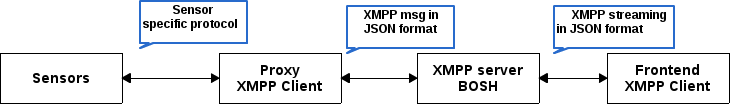
\includegraphics[scale=0.6]{images/Protocol_flow.png}   
      \caption[Protocol flow]{Protocol flow}
      \label{img:protocol}                           
      \end{figure}

      In order to satisfy all aforementioned requirements, two major protocols have been found: \emph{XMPP}\cite{XMPPbook}:a protocol for extensible messaging with a special case of the device-to-server pattern, since people are connected to the servers and \emph{MQTT\footnote{MQ Telemetry Transport, \url{http://mqtt.org/}}}: a protocol for collecting device data and sending it to servers. 

      \textbf{MQTT}
      \newline
      the Message Queue Telemetry Transport, targets device data collection (Fig. \ref{img:MQTT}\footnote{What is MQTT?, \url{https://www.ibm.com/developerworks/}}). As its name states, its main purpose is telemetry, or remote monitoring. Its goal is to collect data from many devices and transport that data to the IT infrastructure. It targets large networks of small devices that need to be monitored or controlled from the cloud.
      \begin{figure}[!ht]
      \centering
      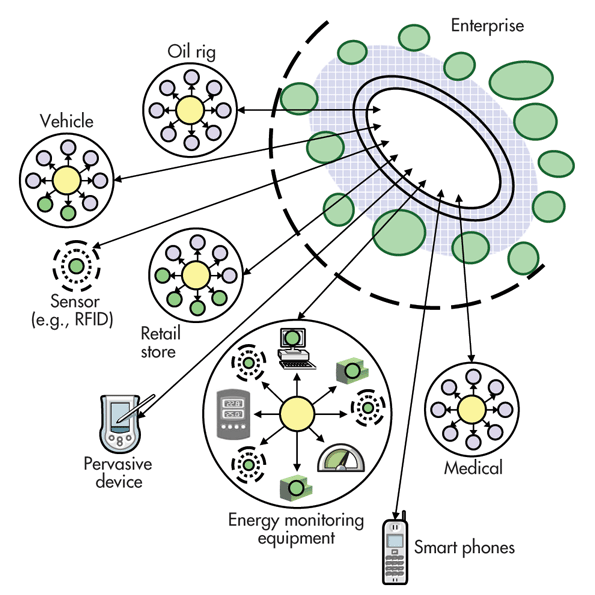
\includegraphics[scale=0.6]{images/MQTT.png}   
      \caption[Message Queue Telemetry Transport]{Message Queue Telemetry Transport}
      \label{img:MQTT}                           
      \end{figure}
      MQTT makes attempt to enable device-to-device transfer, nor to ``fan out'' the data to many recipients. Since it has a clear, compelling single application, MQTT is offering few control options. In this context, ``real time'' for MQTT is typically measured in seconds. All the devices connect to a data concentrator server. So the protocol works on top of TCP, which provides a simple, reliable stream. Since the IT infrastructure uses the data, the entire system is designed to transport data into enterprise technologies.

      MQTT enables applications like monitoring a huge oil pipeline for leaks or vandalism. Those thousands of sensors must be concentrated into a single location for analysis. When the system finds a problem, it can take action to correct that problem. Other applications for MQTT include power usage monitoring, lighting control, and even intelligent gardening. They share a need for collecting data from many sources and making it available to the IT infrastructure.

     \textbf{XMPP}
      \newline 
      XMPP was originally developed for instant messaging (IM) to connect people via text messages (Fig. \ref{img:XMPP}\footnote{IoT, \url{http://electronicdesign.com/embedded/understanding-protocols-behind-internet-things}}). XMPP stands for Extensible Messaging and Presence Protocol. The targeted use is people-to-people communication.
      \begin{figure}[!ht]
      \centering
      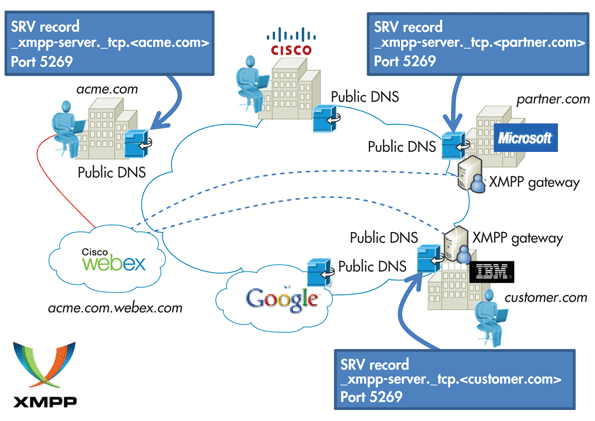
\includegraphics[scale=0.7]{images/XMPP.png}
      \caption[The Extensible Messaging and Presence Protocol (XMPP)]{The Extensible Messaging and Presence Protocol (XMPP)}
      \label{img:XMPP}                           
      \end{figure}

      XMPP uses the XML format messages, making person-to-person communications natural. Like MQTT, it runs over TCP, or over HTTP on top of TCP. Its key strength is a name@domain.com addressing scheme that helps connect the needles in the huge Internet haystack. XMPP powers a wide range of applications including instant messaging, multi-user chat, voice and video conferencing, collaborative spaces, real-time gaming, data synchronization, and even search. Although XMPP started its life as an open, standardized alternative to proprietary instant messaging systems like ICQ and AOL Instant Messenger, it has matured into an extremely robust protocol for all kinds of messaging purposes.

      Most implementations work directly with TCP connections, but \emph{BOSH} extension (bidirectional streams over Synchronous HTTP) lets servers push XMPP data through HTTP long polling sessions, enabling ``real time'' XMPP experience in web-application. Like HTTP, XMPP is a client-server protocol, but it differs from HTTP by allowing either side to send data to the other asynchronously. XMPP connections are long lived, and data is pushed instead of pulled. XMPP has nearly 200 extensions, providing a broad and useful range of tools on which sophisticated applications can be build. 

      After a short research XMPP pecularities clearly show that this protocol can fully satisfy all requirements and be used in generic frontend. So the interface \emph{Data Hub to/from Directory Manager Interface/AuthHandler} will be powered by using XMPP. Thus, it should be discovered in details.
   
      XMPP, like all protocols, defines a format for moving data between two or more communicating entities. In XMPP’s case, the entities are normally a client and a server, although it also allows for peer-to-peer communication between two servers or two clients. Many XMPP servers exist on the Internet, accessible to all, and form a federated network of interconnected systems. Data exchanged over XMPP is in XML, giving the communication a rich, extensible structure. One major feature XMPP gets by using XML is XML's insensibility. This extensibility is put to great use in the more than 200 protocol extensions registered with the XMPP Standards Foundation and has provided developers with a rich set of tools. XML is known primarily as a document format, but in XMPP, XML data is organized as a pair of streams, one stream for each direction of communication. Each XML stream consists of an opening element, followed by XMPP stanzas and other top-level elements, and then a closing element. Each XMPP stanza is a first-level child element of the stream with all its descendant elements and attributes. At the end of an XMPP connection, the two streams form a pair of valid XML documents. The Extensible Messaging and Presence Protocol is the IETF's formalization of the base XML streaming protocols for instant messaging and presence developed within the Jabber community\cite{xmpp}.

      \textbf{Pushing Data}

      HTTP clients can only request data from a server. Unless the server is responding to a client request, it can not send data to the client. XMPP connections, on the other hand, are bidirectional. Either party can send data to the other at any time, as long as the connection is open. This ability to push data expands the possibilities for web applications and protocol design. Instead of inefficient polling for updates, applications can instead receive notifications when new information is available.

      \textbf{Pleasing Firewalls}

      Some web applications support the use of HTTP callbacks, where the web server makes requests to another HTTP server in order to send data. This would be a handy feature to push data if it were not for firewalls, network address translation (NAT), and other realities of the Internet. In practice it is very hard to enable arbitrary connections to clients from the outside world. XMPP connections are firewall and NAT friendly because the client initiates the connection on which server-to-client communication takes place. Once a connection is established, the server can push all the data it needs to the client, just as it can in the response to an HTTP request.
      
      \textbf{Improving Security}

      XMPP is built on top of Transport Layer Security (TLS) and Simple Authentication and Security Layer (SASL) technologies, which provide robust encryption and security for XMPP connections. Though HTTP uses Secure Sockets Layer (SSL), the HTTP authentication mechanisms did not see much implementation or use by developers. Instead, the Web is full of sites that have implemented their own authentication schemes, often badly.
      
      \textbf{Statefulness}

      HTTP is a stateless protocol; XMPP is stateful. Stateless protocols are easier to scale because each server does not need to know the entire state in order to serve a request. This drawback of XMPP is less onerous in practice because most non-trivial web applications make extensive use of cookies, backend databases, and many other forms of stored state. Many of the same tools used to scale HTTP-based applications can also be used to scale XMPP-based ones, although the number and diversity of such tools is more limited, due to XMPP’s younger age and lesser popularity.

      Main XMPP properties are:
      \begin{itemize}
      \item \emph{Decentralization}. The architecture of the XMPP network is similar to email; anyone can run their own XMPP server and there is no central master server.
     \item \emph{Open standards}. The Internet Engineering Task Force has formalized XMPP as an approved instant messaging and presence technology under the name of XMPP (the latest specifications are RFC 6120 and RFC 6121). No royalties are required to implement support of these specifications and their development is not tied to a single vendor.
      \item \emph{History}. XMPP technologies have been in use since 1999. Multiple implementations of the XMPP standards exist for clients, servers, components, and code libraries.
      \item \emph{Security}. XMPP servers can be isolated from the public XMPP network (e.g., on a company intranet), and strong security (via SASL and TLS) has been built into the core XMPP specifications.
      \item \emph{Flexibility}. Custom functionality can be built on top of XMPP; to maintain interoperability, common extensions are managed by the XMPP Standards Foundation. XMPP applications beyond IM include group chat, content syndication, collaboration tools, file sharing, gaming, remote systems control and monitoring of geolocation, cloud computing, VoIP and Identity services.
      \end{itemize}

      \begin{figure}[!ht]
      \centering
      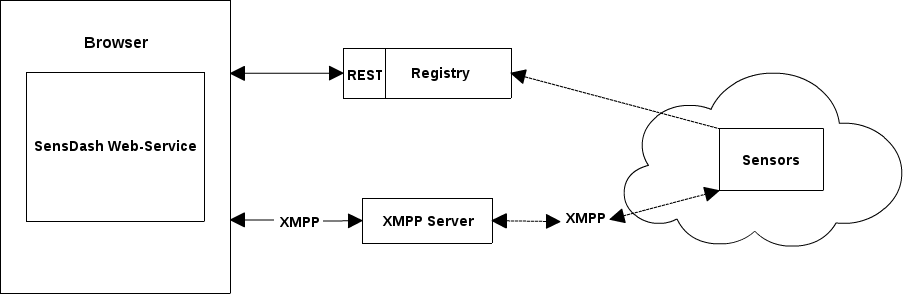
\includegraphics[scale=0.5]{images/Interface.png}   
      \caption[Interface]{Interface}
      \label{img:interfaces}                           
      \end{figure}

      The XMPP network uses a client-server architecture (clients do not talk directly to one another). However, it is decentralized by design, there is no central authoritative server. Anyone may run their own XMPP server on their own domain. Every user on the network has a unique Jabber ID (usually abbreviated as JID). To avoid requiring a central server to maintain a list of IDs, the JID is structured like an email address with a username and a domain name (or IP address) for the server where that user resides, separated by an at sign (@), such as username@example.com.  

\subsection{Backend Entry Points}
    Data Hub and Registry are two modules that have been standardized by frontend and have to be fully implemented on a backend side. Since both of these parts support common standards such as Web API, AJAX, JSON or XML file format, it makes possible to implement every functional module on a backend side without dependency on OS type, framework or language of implementation. Separation between metadata and streaming data increase scalaility of a system, such that any number of Registries and Data Hubs can be deployed in runtime. Defined Web API and XMPP-based interfaces between frontend's and backend's sides based on open standards. In case of XMPP-based interface, all communication are flows through a distributed XMPP network. Thus, Data Hub needs to have its own XMPP server or sends a requests through any alternative server.

\section{Data Tier}
   As was mentioned in the Section 4.1 data tier contains data sources that have to be retrieved via application tier to a client tier. Data tier consists of hardware and software sensors, which provide information to a user. The data format which can be retrieved by frontend via XMPP connection has no limitation, but in scope of this master thesis such type of information was defined as text and hashmap of values. Text format is used as an example of information provided by software sensor. In the same time hardware sensor periodically sends measured map o values. These types of data changes with some time-frequency and automatically retrieved by the client tier as a real-time data stream.

  An important aspect in streaming data that some of data can be cashed on a server side, thus become possible to retrieve data after it was produced. But sometimes relevant data has to be live, thus there is no other options except of live streaming, where the connection configuration, aliveness and quality become a key aspect. All these properties are already covered by XMPP. Considering the absence of any concrete backend system, cashing of a data can be done based on XMPP server configuration. 

  \textbf{Sensor Functional Characteristics}
  \newline
  An essential part of a concept is to guarantee reliable and secure data transportation. Thus, every data source can acquire additional properties based on a system architecture:
  \begin{itemize}
  \item reliability
  \item perfomance
  \item security
  \end{itemize}
  All these three characteristics rely on a quantity of available Data Hubs which include XMPP modules and handle data streaming. Since Data Hub has to provide data from sensor to frontend by using XMPP connection, it has to support XMPP data channel configurations and may play a role of end-point for frontend. If sensor has 2 end-points it should be mentioned in Registry together with a type of data transfer protocol (covered in the Section 5.2).

  A simple sensor with a low level of reliability has only a single end-point (Figure~\ref{img:end_points}~a). A reliable sensor has two, where first one is primary, and next serves as backup/failover (Figure~\ref{img:end_points}~c). A highly reliable sensor has three or more end-points, which guarantee data delivery in case of n-1 endpoints failing. 
     \begin{figure}[!ht]
     \centering
     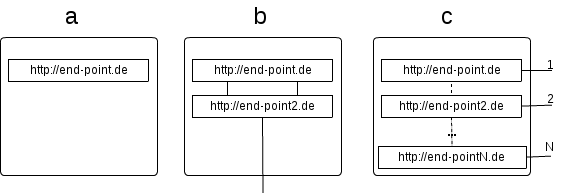
\includegraphics[scale=0.6]{images/FuncCharacteristics.png}   
     \caption[MVC Pattern]{Sensor Functional Characteristics} 
     \label{img:end_points}                     
     \end{figure}
A high-performance sensor has two or more end-points (Figure \ref{img:end_points}~c) working in parralell. In contrast to reliability end-points, high performance does not perform failovers, using all endpoints in the same time to achieve better bandwith and minimize latency.

A secure sensor should be maintained by at least two end-points, each transporting an unrecoverable part of a data (Figure~\ref{img:end_points} b). This way, even by compromising some of endpoints, a full message could not be stolen. 

All functional characteristics of sensors should be automatically retrieved by frontend from predefined attributes located in Registries. Users then would be able to estimate conditions and quality of data streams before subscribing to them. Frontend should have a logic which calculates a number sensor end-points, analyses their basic characteristics and graphically represents it using icons and labels, presenting most important technical metadata in a user-friendly way. In case of end-point problems, frontend should automatically perform a failover to the next available endpoint, if it exists. Developers that want want to use generic frontend as a proxy for their application, should care about correct ordering of end-points, and pay attention to connection process in order to provide high-secure, reliable and high-performance data retrieval.

\section{Summary}
	In this chapter, according to a 3-tier architecture, the first web-based concept for sensor streaming services has been created. Fine-grained structure provides clear separation of concerns between different modules of the concept. The client tier consists of GUI content and client framework; the application tier provides an application logic to interconnect backend and client tier; and finally, the data tier describes format of a data in order to easily connect it with the application tier and visually represent it by using the client tier. Every data souce was assigned such functional characteristics as reliability, perfomance and security level of information streams. Every characteristic relies on a number of end-points responsible for sensor. 

  As a result a fine-grained structure of the concept was built on top of next modules: 
  
  Registry responsibilities:
  \begin{itemize}
  \item stores an metadata about available sensors registered in the network;
  \item provides HTTP Web API in JSON format.
  \end{itemize}
  
  Data Hub responsibilities:
  \begin{itemize}
    \item be aware of metadata provided by the Registry;
    \item bind metadata from the Registry with real-time data streaming from a sensor;
    \item get and parse sensor streaming data and reconvert sensor-specific protocol to XMPP;
    \item implement XMPP services and guarantee message exchange between the frontend and sensors;
    \item store history of data sources and personal user preferences.
  \end{itemize}

  Web-server responsibilities: handles delivery of static web content.

  Frontend responsibilities:
  \begin{itemize}
  \item interconnect all modules by using appropriate interfaces: Web API for Registry and XMPP interface for Data Hub and AuthHandler;
  \item build a responsive and adaptive GUI;
  \item implement a scalable and efficient system structure (adding new Registries/sensors through a web form, changing personal preferences, and other typical frontend functions should productive, user-friendly, and easily extensible).
  \end{itemize}
	%!TEX root = Thesis.tex
\chapter{Implementation and Evaluation}
	The chapter contains practical part of the work, describing implementation of suggested prototype in the section
	2.3. The prototype implements the major aspects proposed in the concept (chapter 4).
	The implementation consists the major aspects proposed in the concept, according to 3-tier architecture. Namely next components:
	 \begin{itemize}
		\item \textbf{Client Tier} presents adaptive to different screens GUI, dynamically changed content and multy-user access
		\item \textbf{Application Tier} consists Apache Web-server, XMPP server and garantee appropriate interface of collaboration between iers via JSON format and defined structure
		\item \textbf{Data Tier} consists cookies for authorization
	\end{itemize}
	To make evaluations real, system will use data from the VICCI(Visual and Interactive Cyber-physical Systems Control and Integration) project at the Faculty of Computer Science of the Dresden University of Technology. The scope includes smart home environments and supporting people in the ambient assisted living. Also it was connected by using Data Hub as a Proxy, that is the part of Master Thesis of Luiz Alberto Borges, "Data Hub for Adaptive Data Services".
%%%%%%%%%%%%%%%%%%%%%%%%%%%%%%%%%%%
\section{Develpment Environment}
	As a programming languages for implementation of this work jQuery\footnote{jQuery programming language, \url{http://jquery.com/}} and HTML5 together with CSS3 are chosen. jQuery is a fast, small, well documented, easy to use, widely-used and feature-rich JavaScript library. In addition it has such an important properties as: chaining, easy-to-use AJAX, event handlers, CSS selectors, pluins. It makes things like HTML document traversal and manipulation, event handling, animation, and Ajax much simpler with an easy-to-use API that works across a multitude of browsers.It enables the project code to be portable over different platforms and provides opportunity for robust and effective development. The choice is dictated mostly by two aspects. On the one hand, the system that is being developed is distributed by it’s nature. On the other hand, jQuery has low entry barrier, and the code written in this language is extremely readable, laconic and understandable. These facts make further support of written code much easier for other developers that have an experience with any other JavaScript library.
	\newline
	\begin{table}[H]
	\centering
	\begin{tabular}{|r|l|l|l|l|l|}
	\hline
	Target 			& jQuery & Dojo & Prototype & YUI & ExtJS \\
	\hline
	\hline
	License		& MIT & BSD \& AFL & MIT & BSD & GPL and Commercial \\
	\hline
	Size		& 32 KiB & 41 kB & 46–278 kB & 31 kB & 84–502 kB \\
	\hline
	Source language		& JavaScript & JavaScript + HTML & JavaScript &  Javascript + HTML + CSS & JavaScript \\
	\hline
	Grid		& yes & yes & yes & - & yes  \\
	\hline
	DOM wrapped		& yes & yes & yes & no & yes \\
	\hline
	Other data retrieval		& XML,HTML & XML,HTML,CSV,ATOM & - & yes & XML  \\
	\hline
	DOM wrapped		& yes & yes & yes & no & yes \\
	\hline
	Server push data retrieval		& yes & yes & - & via Plugin & yes \\
	\hline
	GUI page layout		& with Plugin & yes & yes & - & yes \\
	\hline 		
	Touch events		& with Plugin & yes & yes & - & yes \\
	\hline 
	\end{tabular}
	\caption[Caption in TOC]{Comparison of JavaScript frameworks}
	\label{tab:JS_frameworks}
	\end{table}
	Also the most important part is a version of browser support. jQuery\footnote{jQuery browser support, \url{http://jquery.com/browser-support/}}, Dojo\footnote{Dojo browser support,\url{http://livedocs.dojotoolkit.org/releasenotes/1.4}}, Prototype\footnote{Prototype browser support, \url{http://prototypejs.org/doc/latest/Prototype/Browser/index.html}} , YUI\footnote{YUI browser support, \url{http://yuilibrary.com/yui/environments/}}, ExtJS\footnote{ExtJS browser support, \url{http://www.sencha.com/products/extjs/}}

	\begin{table}[H]
	\centering
	\begin{tabular}{|r|l|l|l|l|l|}
	\hline
	Target 			& jQuery & Dojo & Prototype & YUI & ExtJS \\
	\hline
	\hline
	Chrome		& 1+ & 3 & 1+ & - & 10+ \\
	\hline
	Opera		& 9+ & 10.50+ & 9.25+ & 10.0+ & 11+ \\
	\hline
	Safari		& 3+ & 4 & 2.0.4+ & 4.0 & 4+ \\
	\hline
	Mozilla Firefox		& 2+ & 3+ & 1.5+ & 3+ & 3.6+ \\
	\hline
	Internet Explorer		& 6+ & 6+ & 6+ & 6+ & 6+ \\
	\hline
	\end{tabular}
	\caption[Caption in TOC]{Browser Support}
	\label{tab:internal_results}
	\end{table}


\section{Web-based Framework Analysis}
 \begin{itemize}
	\item \textbf{Bootstrap}
	\newline
	Bootstrap is the most popular and widely used framework, nowadays. It’s a beautiful, intuitive and powerful web design kit for creating cross browser, consistent and good looking interfaces. It offers many of the popular UI components with a plain-yet-elegant style, a grid system and JavaScript plugins for common scenarios.

	It consists of four main parts:
	Scaffolding – global styles, responsive 12-column grids and layouts. Bear in mind that Bootstrap doesn’t include responsive features by default. If design needs to be responsive this functionality have to be done manually. Base CSS – this includes fundamental HTML elements like tables, forms, buttons, and images, styled and enhanced with extensible classes. Components – collection of reusable components like dropdowns, button groups, navigation controls (tabs, pills, lists, breadcrumbs, pagination), thumbnails, progress bars, media objects, and more. JavaScript – jQuery plugins which bring the above components to life, plus transitions, modals, tool tips, popovers, scrollspy (for automatically updating nav targets based on scroll position), carousel, typeahead (a fast and fully-featured autocomplete library), affix navigation, and more.
	\item \textbf{Foundation}
	\newline
	Foundation is a powerful, feature-rich, responsive front-end framework. With Foundation user can quickly prototype and build websites or apps that work on any kind of device, with tons of included layout constructs, elements and best practices. It’s built with mobile first in mind, utilitizes semantic features, and uses Zepto instead of jQuery in order to brings better user experience and faster performance.

	Foundation has a 12-column flexible, nestable grid powerful enough to create rapidly multi-device layouts. In terms of features it provides many. There are styles for typography, buttons, forms, and various navigation controls. Many useful CSS components are provided like panels, pricing tables, progress bars, tables, thumbnails, and flex video that can scale properly your video on any device. And, of course, JavaScript plugins including dropdowns, joyride (a simple and easy website tour), magellan ( a sticky navigation that indicates where is the user on the page), orbit (a responsive image slider with touch support), reveal (for creating modal dialogs or pop-up windows),  sections (a powerful replacement for traditional accordions and tabs), and tooltips.
	\item \textbf{GroundworkCSS}
	\newline
	GroundworkCSS is a new, fresh addition to the front-end frameworks family. It’s a fully responsive HTML5, CSS and JavaScript toolkit built with the power of Sass and Compass which gives the ability to rapidly prototype and build websites and apps that work on virtually any device.

	It offers an extremely flexible, nestable, fraction-based, fluid grid system that makes creating any layout possible. GroundworkCSS has some really expressive features like tablets and mobile grids which maintain the grid column structure instead of collapsing the grid columns into individual rows when the viewport is below 768 or 480 pixels wide. Another cool feature is a jQuery ResponsiveText plugin which allows to have dynamically sized text that adapts to the width of the viewport: extremely useful for scalable headlines and building responsive tables.
	The framework includes a rich set of UI components like tabs, responsive data tables, buttons, forms, responsive navigation controls, tiles (a beautiful alternative to radio buttons and other boring standard form elements), tooltips, modals, Cycle2(a powerful, responsive content slider), and many more useful elements and helpers. It also offers a nice set of vector social icons and a full suite of pictographic icons included in FontAwesome. To see the framework in action user can use the resizer at the top center of the browser window. This way user can test the responsiveness of the components against different sizes and viewports while exploring the framework’s features. GroundworkCSS is very well documented with many examples, and to get user started quickly the framework also provides several responsive templates. The only thing as a weakness is the missing of a way to customize download.

	\item \textbf{Gumby}            
	\newline
	Gumby is simple, flexible, and robust front-end framework built with Sass and Compass.

	Its fluid-fixed layout self-optimizes the content for desktop and mobile resolutions. It support multiple types of grids, including nested ones, with different column variations. Gumby has two PSD templates that get user started designing on 12 and 16 column grid systems.
	The framework offers feature-rich UI Kit which includes buttons, forms, mobile navigation, tabs, skip links, toggles and switches, drawers, responsive images, retina images, and more. Following the latest design trends the UI elements have Metro style flat design but can use Pretty style with gradient design too, or to mix up both styles. An awesome set of responsive, resolution independent Entypo icons, is completely integrated into the Gumby Framework. Gumby has also a very good customizer with color pickers which helps to build your custom download with ease.
	\item \textbf{Kube}
	\newline
	Lastly, if user need a solid, yet simple base without needless complexity and extras, for your new project, Kube can be the right choice. Kube is a minimal, responsive and adaptive framework with no imposed styling which gives to user the freedom to create. It offers basic styles for grids, forms, typography, tables, buttons, navigation, and other stuff like links or images.

	The framework contains one compact CSS file for building responsive layouts with ease and two JS files for implementing tabs and buttons in your designs. If user is looking for maximum flexibility and customization, user can download developer version which includes LESS files, with variables, mixins and modules.
	\end{itemize}

\begin{figure}[!ht]
\centering

\includegraphics[scale=0.7]{images/Bootstrap&Foundation.png}
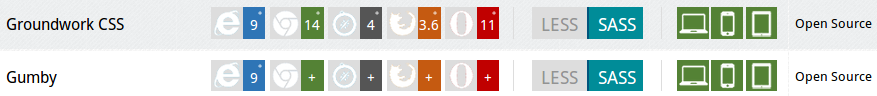
\includegraphics[scale=0.7]{images/Groundwork&Gumby.png} 

\includegraphics[scale=0.7]{images/Kube.png}  
\caption[Framework Comparison]{Framework Comparison\footnote{\url{http://usablica.github.io/front-end-frameworks/compare.html}}}
\label{img:Bootstrap&Foundation.png}
\label{img:Groundwork&Gumby.png}   
\label{img:Kube.png}                          
\end{figure}

\section{Data Flow Model}
	\subsection{XMPP BOSH Client}
	The Extensible Messaging and Presence Protocol (XMPP) is the IETF’s formalization of the base XML streaming protocols for instant messaging and presence developed within the Jabber community starting in 1999. This page provides a brief chronology of Jabber/XMPP technologies from the perspective of standardization\cite{xmpp}.
		\newline
	\emph{Decentralization}
	\newline
	The architecture of the XMPP network is similar to email; anyone can run their own XMPP server and there is no central master server.
	\newline
	\emph{Open standards}
	\newline
	The Internet Engineering Task Force has formalized XMPP as an approved instant messaging and presence technology under the name of XMPP (the latest specifications are RFC 6120 and RFC 6121). No royalties are required to implement support of these specifications and their development is not tied to a single vendor.
	\newline
	\emph{History}
	\newline
	XMPP technologies have been in use since 1999. Multiple implementations of the XMPP standards exist for clients, servers, components, and code libraries.
	\newline
	\emph{Security}
	\newline
	XMPP servers can be isolated from the public XMPP network (e.g., on a company intranet), and strong security (via SASL and TLS) has been built into the core XMPP specifications.
	\newline
	\emph{Flexibility}
	\newline
	Custom functionality can be built on top of XMPP; to maintain interoperability, common extensions are managed by the XMPP Standards Foundation. XMPP applications beyond IM include groupchat, network management, content syndication, collaboration tools, file sharing, gaming, remote systems control and monitoring, geolocation, middleware and cloud computing, VoIP and Identity services.
	The XMPP network uses a client–server architecture (clients do not talk directly to one another). However, it is decentralized—by design, there is no central authoritative server, as there is with services such as AOL Instant Messenger or Windows Live Messenger. Some confusion often arises on this point as there is a public XMPP server being run at jabber.org, to which a large number of users subscribe. However, anyone may run their own XMPP server on their own domain.
	Every user on the network has a unique Jabber ID (usually abbreviated as JID). To avoid requiring a central server to maintain a list of IDs, the JID is structured like an email address with a username and a domain name (or IP address[16]) for the server where that user resides, separated by an at sign (@), such as username@example.com.

\section{Browser Support}
	In past years a Flash-based media player in more than sufficient for streaming on the Web and this technology is still necessary to support legacy browsers. But thankfully modern standards have advanced and the inclusion of HTML5 video opens doors for dozens of new opportunities.

	In this guide I’d like to offer an introduction to HTML5 video for the Web. It will take some practice to understand the native in-browser player and all its functionality. When you’re working with a flash video player it’s all too common to associate all video formats in .flv. While this does work, most flv files cannot retain quality anywhere near the more advanced file formats/codecs. There are 3 important video types which are supported by HTML5: MP4, WebM, and Ogg/Ogv. The MPEG-4 file type is generally encoded in H.264 which allows for playback in third party Flash players. This means you don’t need to keep a .flv video copy to support a fallback method! WebM and Ogg are two much newer file types related to HTML5 video. Ogg uses Theora encoding which is based on the open-source standard audio file format. These can be saved with a .ogg or .ogv extension.
	So which of these file types do you need for your website? Well ideally all 3 would be great as they provide the full support spectrum. Yet this isn’t realistic, and in fact, you can cover all the bases with only two of them. Here is a breakdown of what works for each browser:

	Mozilla Firefox – WebM, Ogg
	Google Chrome – WebM, Ogg
	Opera – WebM, Ogg
	Safari – MP4
	Internet Explorer 9 – MP4
	Internet Explorer 6-8 – No HTML5, Flash Only!
	Most flash video players will support MP4 files as long as they’re encoded in H.264. As such, each of these browsers will embed MP4+Flash as a final resort. This means you only need to create two different video formats to support all browsers. MP4 for Safari/IE9 and a choice between WebM or Ogg for the rest.

\section{Database Model}

\section{Use Cases}

  \subsection{Frontend}
  \subsection{3-tier Architecture in Software Projection}
    \subsection{Use Cases Realization}
  \subsection{Evaluation}


\subsection{Summary}
	%!TEX root = Thesis.tex
\chapter{Conclusion and Outlook}

\section{Conclusion}
The chapter summarizes the presented thesis providing an overview of each chapter
and describing the achievement of the thesis’s goals defined in the section 1.2. At
the end of the chapter suggestions for the future work are made.
\subsection{Addressed research questions}

\subsubsection{Achieved Goals}

\begin{itemize}
\item Some;
\item Statements;
\item Here;
\end{itemize}

Finally, a statement\footnote{With footnote, \url{www.and-some-url}}

\subsection{Practical results}

\section{Future work}
To conclude the thesis, suggestions for the future work are made. These suggestions
are devoted to improve either the developed concept or the current implementation.
\newline
Visualization and interaction metaphor for the introduced access control
\newline
Enhanced user interface for application part
\newline
User interface to support the introduced dynamic composition

  \listoffigures
    \addcontentsline{toc}{chapter}{List of Figures}
  \listoftables
    \addcontentsline{toc}{chapter}{List of Tables}
  \printglossary[type=\acronymtype,style=long,title=List of Abbreviations,toctitle=List of Abbreviations]
  \bibliography{bibliography}
\end{document}
